\section{Point Kinetics/Lumped Thermal Hydraulics}
\label{sec:pointkinetics_th}

\subsection{Problem Statement}
\label{subsec:pointkinetics_th_ps}

A reduced order model based on the anchored-\ac{ANOVA} decomposition will be constructed in this section for a simple system of ordinary differential equations modeling a transient in a BN800 sodium fast cooled reactor. The physical model of the reactor consists of point kinetics to model the neutronics and lumped thermal hydraulics equations to describe temperature feedback. The coupled system is nonlinear and only has a time dependence. Previous research groups have utilized point kinetics and lumped thermal hydraulics equations to model basic reactor systems in \cite{Gilli_annals}, \cite{Gilli_mc2011}, and \cite{Housiadas}. In this section a reduced order model will be constructed for the maximum fuel temperature attained following a reactivity insertion as a function of the random variables exhibited in the description of the point kinetics/lumped thermal hydraulics system.  

The six-group point kinetics equations modeling the neutronics of a reactor consist of a balance for reactor power $P(t)$ and a balance equation for each of the six precursor concentrations $C_k(t)$. Changes in reactor power are dependent on the precursor concentration, decays constants $\lambda_k$, delayed neutron fraction $\beta$ and the mean neutron generation time $\Lambda$ as detailed in,
\begin{equation}
\label{eq:pk_power}
   \frac{dP}{dt} = \frac{\rho(T_f,T_c,t)-\beta}{\Lambda}P +
    \sum_{k=1}^6 \lambda_k C_k.
\end{equation}  
The reactivity $\rho$ depends on feedback from the fluids temperature models for the reactor fuel and coolant, which in turn depend on reactor power. The expression for each of the $k$ precursor concentrations is written as,
\begin{equation}
\label{eq:pk_precursors}
   \frac{dC_k}{dt} = -\lambda_k C_k +
    \frac{\beta_k}{\Lambda}P.
\end{equation}
As for the ordinary differential equations describing the behavior of the reactor coolant system, two coupled equations suffice. For the fuel temperature $T_f$, the following lumped model is used,
\begin{equation}
\label{eq:pk_fuel}
   M_f c_{pf}\frac{dT_f}{dt} = P + Ah(T_c-T_f)
\end{equation}
where $M_f$ is the lump fuel mass, $c_{pf}$ is the specific heat capacity of the fuel, $A$ is the heat transfer surface, and $h$ is the heat transfer coefficient between the coolant and reactor fuel. Finally, the coolant temperature is described as,
\begin{equation}
\label{eq:pk_coolant}
   M_c c_{pc}\left(\frac{dT_c}{dt} +v \frac{T_c - T_{in}}{L}\right) = 
    Ah(T_f-T_c)
\end{equation}
where $M_c$ is the lump coolant mass, $c_{pc}$ is the specific heat capacity of the coolant, $L$ is the coolant channel length, $v$ is the coolant flow velocity, and $T_{in}$ is the inlet coolant temperature. The initial conditions for $P$, $C_k$, $T_f$, and $T_c$ depend on the initial power in the reactor $P_0$ before any kind of transient occurs and are listed in \ref{eq:pk_initial_conds}. 
\begin{eqnarray}
\label{eq:pk_initial_conds}
   P(0) &=& P_0 \\ 
   C_k(0) &=& \frac{\beta_k}{\lambda_k\Lambda}P_0 \nonumber \\
   T_f(0) &=& T_c(0) + \frac{P_0}{Ah} \nonumber \\
   T_c(0) &=& T_{in} + \frac{P_0L}{M_c c_{pc}v} \nonumber
\end{eqnarray}
Serving as the coupling device between the lumped thermal hydraulics model and point kinetics model is the reactivity, which is proportional to the coolant temperature and the fuel temperature. Of course, any external reactivity $\rho_{ex}$ added to the reactor is also a contributor. The time dependent reactivity is given explicitly as,
\begin{equation}
\label{eq:pk_reactivity}
   \rho(T_f,T_c,t) = \rho_{ex} + \alpha_d(T_f - T_f(0))
    + \alpha_c(T_c - T_c(0))
\end{equation}
where $\alpha_d$ and $\alpha_c$ are the doppler and coolant coefficients of reactivity, respectively.  

The equations in \ref{eq:pk_power}, \ref{eq:pk_precursors}, \ref{eq:pk_coolant}, and \ref{eq:pk_fuel} are used to model the transient resulting from a half sawtooth external reactivity insertion, as shown in \ref{eq:pk_half_sawtooth}. 
\begin{equation}
\label{eq:pk_half_sawtooth}
   \rho_{ex}(t) = \left\{
    \begin{array}{cr}
     t\rho_{max}/20 & t \leq 20 \\
     0                      & t > 20 
    \end{array}
    \right.
\end{equation}
By treating the coefficients in the point kinetics/lumped thermal hydraulics model as random variables, the objective function investigates the response surface for the maximum fuel temperature attained during transient. The reduced order methodologies will be tested against the stated problem. A depiction of the transient at the random variables' mean values, along with the external reactivity is shown in Figure \ref{fig:pk_transient}.  
\begin{figure}
\caption{ \label{fig:pk_transient}
Transient resulting from a half sawtooth external reactivity insertion, as modeled using the mean parameter values of the point kinetics/lumped thermal hydraulics system.}
 \begin{center}
  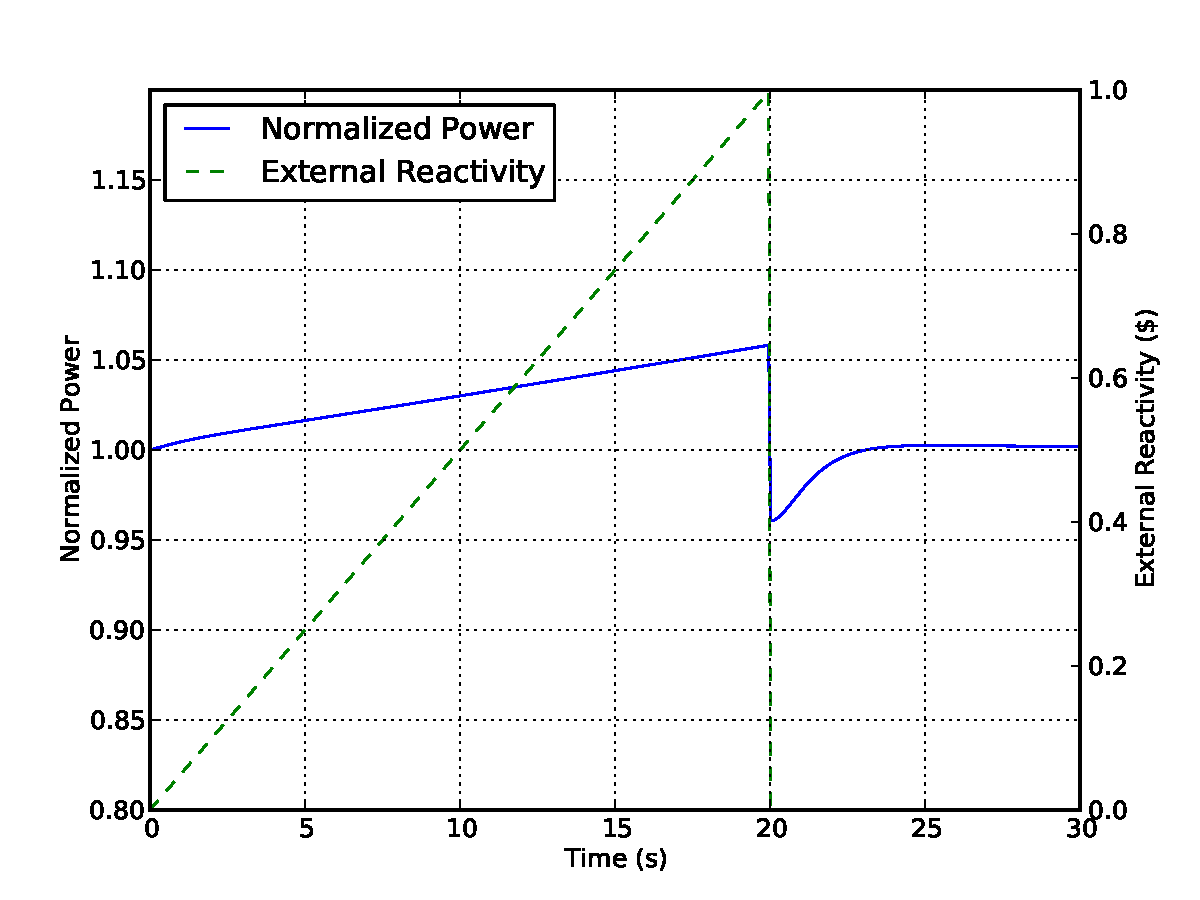
\includegraphics[scale=.75]{./Chapter3/pk_power.pdf}
 \end{center}
\end{figure}
A total of twenty two random variables will be investigated for their affect on the maximum fuel temperature attained during transient. The random variables' mean values, along with their standard deviations are listed in \ref{table:pkinetics_parameters}. Note that all standard deviations are taken to be 5\% of the mean value. All random variables are assumed to be independent of one another, as was assumed in \cite{Gilli_mc2011}. 
\begin{table} 
\caption{\label{table:pkinetics_parameters} 
Mean parameter values used in the point kinetics/lumped thermal hydraulics model for the analysis of a BN800 fast sodium cooled reactor.}
\centering
\begin{tabular}{||c|c|c|c||} 
\hline \hline
\textbf{Random Variable} & \textbf{Units} & \textbf{Mean} & \textbf{Standard Dev.} \\ \hline
$\lambda_1$  &  $s^{-1}$      &  1.24E-02  &  6.20e-04  \\ \hline
$\lambda_2$  &  $s^{-1}$      &  3.05E-02  &  1.52e-03  \\ \hline
$\lambda_3$  &  $s^{-1}$      &  1.11E-01  &  5.55e-03  \\ \hline
$\lambda_4$  &  $s^{-1}$      &  3.01E-01  &  1.50e-02  \\ \hline
$\lambda_5$  &  $s^{-1}$      &  1.14E+00  &  5.70e-02  \\ \hline
$\lambda_6$  &  $s^{-1}$      &  3.01E+00  &  1.50e-01  \\ \hline
$\beta_1$    &                &  9.00E-05  &  4.50e-06  \\ \hline
$\beta_2$    &                &  8.53E-04  &  4.26e-05  \\ \hline
$\beta_3$    &                &  7.00E-04  &  3.50e-05  \\ \hline
$\beta_4$    &                &  1.40E-03  &  7.00e-05  \\ \hline
$\beta_5$    &                &  6.00E-04  &  3.00e-05  \\ \hline
$\beta_6$    &                &  5.50E-04  &  2.75e-05  \\ \hline
$\Lambda$    &  $s$           &  4.00E-07  &  2.00e-08  \\ \hline
$Ah$         &  $kW/K$        &  2.50E+06  &  1.25e+05  \\ \hline
$M_c$        &  $kg$          &  1.16E+03  &  5.84e+01  \\ \hline
$M_f$        &  $kg$          &  9.67E+03  &  4.83e+02  \\ \hline
$c_{pc}$     &  $J/kg\cdot K$ &  1.20E+03  &  6.00e+01  \\ \hline
$c_{pf}$     &  $J/kg\cdot K$ &  5.00E+02  &  2.50e+01  \\ \hline
$v$          &  $m/s$         &  7.50E+00  &  3.75e-01  \\ \hline
$\alpha_d $  &  $pcm/K$       &  6.87E-06  &  3.43e-07  \\ \hline
$\alpha_c$   &  $pcm/K$       &  1.23E-06  &  6.15e-08  \\ \hline
$\rho_{max}$ &                &  4.19E-04  &  2.09e-05  \\ 
\hline \hline
\end{tabular}
\end{table}
A plot of the fuel temperature as a function of time due to the external reactivity profile shown in the same figure is depicted in Figure \ref{fig:pk_fuel_temp}. 
\begin{figure}[!htb]
\caption{ \label{fig:pk_fuel_temp}
Fuel temperature transient resulting from a half sawtooth reactivity insertion. All parameters in the coupled point kinetics/lumped thermal hydraulics equations are held at their mean values. 
}
 \begin{center}
  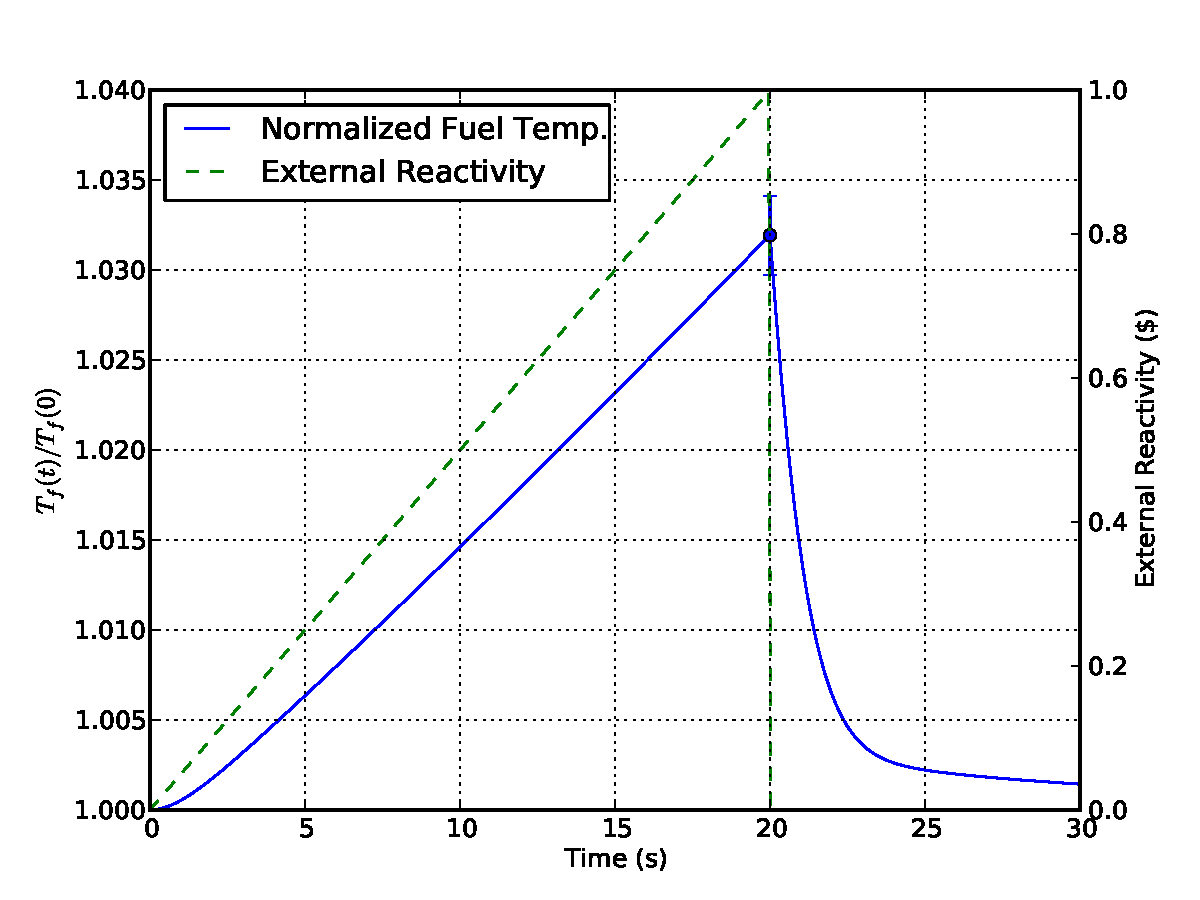
\includegraphics[scale=.75]{./Chapter3/pk_fueltemp.pdf}
 \end{center}
\end{figure}

\subsection{Analysis}
\label{subsec:pointkinetics_th_analysis}

An adaptive reduced order model, whose formulation is summarized in Algorithm \ref{code:rom_algorithm}, will be created for the problem described in section \ref{subsec:pointkinetics_th_ps}. The reduced order model will be investigated for its ability to reproduce statistics of interest by comparing its results with those obtained from sampling the true function. As described in Algorithm \ref{code:rom_algorithm}, the first step in creating a reduced order model for the maximum fuel temperature is to construct all first order components in the anchored-\ac{ANOVA} decomposition and to identify the important ones. The sparse grids comprising the reduced order model are assumed to be converged when the maximum hierarchical surplus for a given level is less than $10^{-5}$. Consequently, at least five digits of accuracy are expected. Important dimensions are those whose normalized sensitivity index in Eq. \ref{eq:anova_sensitivity} exceeds 5\%.

From Figure \ref{fig:pk_importance_pie} the "important" variables are identified to be $Ah$, $\alpha_d$, and $\rho_{max}$. Collectively these three "important" random variables comprise 82\% of the total sensitivity. 
\begin{figure}[!htb]
\caption{ \label{fig:pk_importance_pie}
Normalized sensitivity indices for all random variables comprising the coupled point kinetics/lumped thermal hydraulics equations. The effects of all $\beta_k$ and $\lambda_k$ have been lumped into single $\beta$ a $\lambda$ effects, respectively. 
}
 \begin{center}
  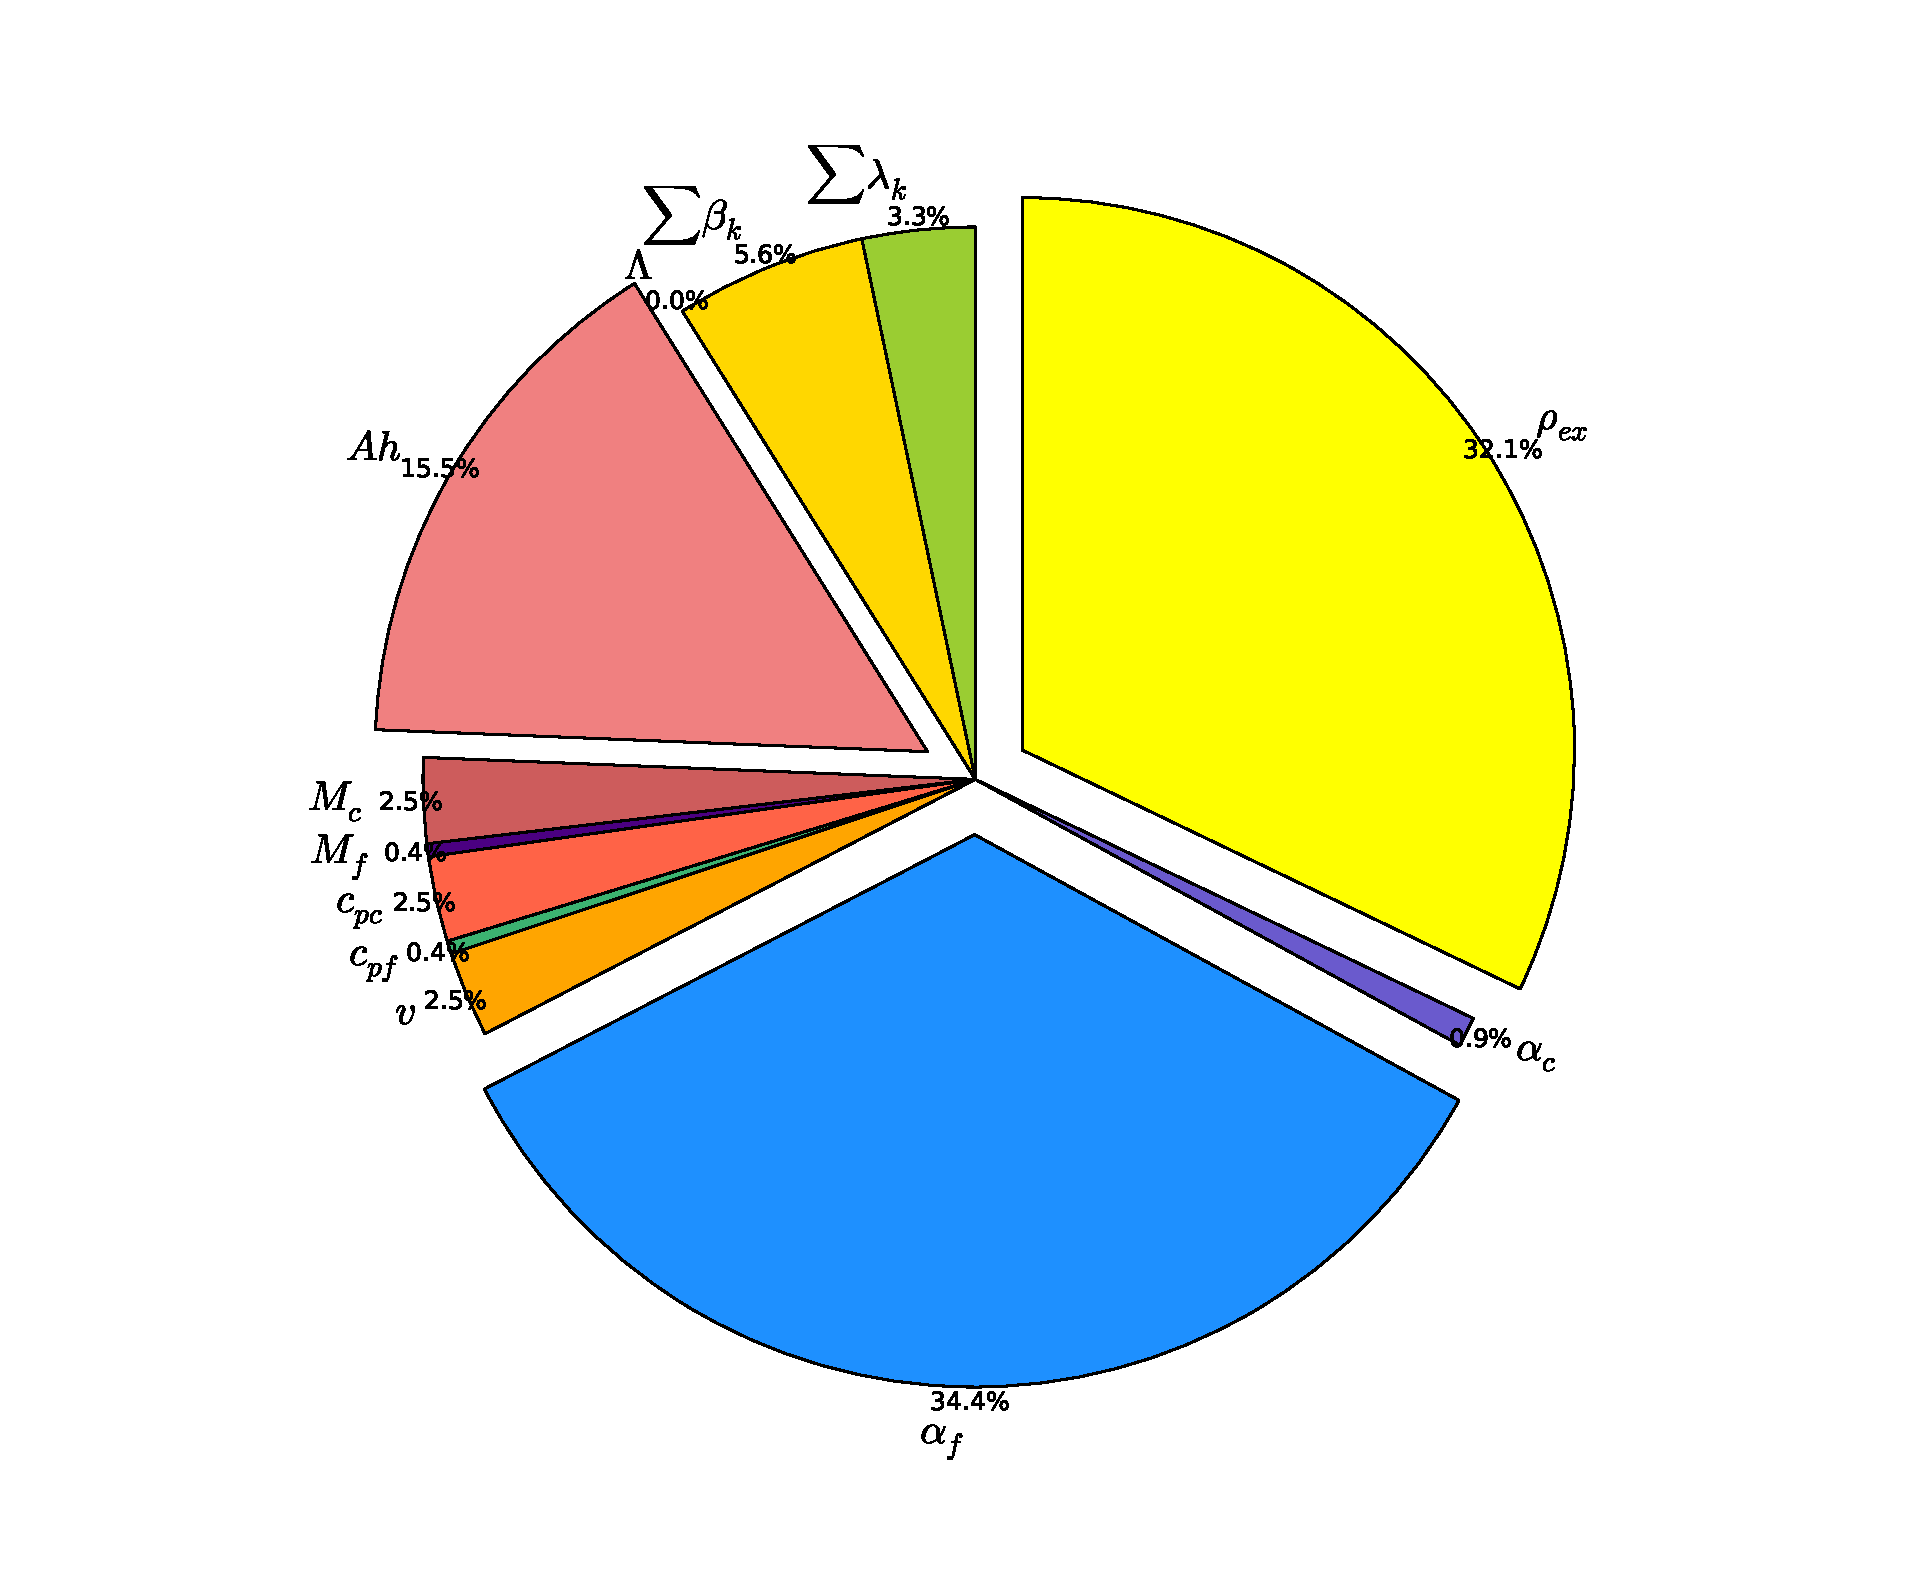
\includegraphics[scale=.5]{./Chapter3/pk_importance_pie.pdf}
 \end{center}
\end{figure}
The indication that the maximum fuel temperature is sensitive to the heat transfer $Ah$ from fuel to coolant is not surprising since in Eq. \ref{eq:pk_fuel} the fuel temperature is directly proportional to $Ah$. Further, the random variables $\rho_{max}$ and $\alpha_d$ determine the slope of the increase in fuel temperature, as seen in Figure \ref{fig:pk_fuel_temp}, and so a strong sensitivity to these random variables is expected. The sensitivity of the maximum fuel temperature to $\alpha_c$ is not as great since the increase in coolant temperature during the transient is significantly smaller than the rise in fuel temperature. Relatively weak sensitivity to $M_f$ and $c_{pf}$ can perhaps be attributed to cancellation of error since these two variables are multiplied together.

With only three random variables deemed as "important" only three second order anchored-\ac{ANOVA} components must be built for the reduced order model. Neglecting any convergence criteria, third order component describing the interaction effects among the three important random variables is also built. A summary of the total number of function evaluations needed to construct the adaptive reduced order model for the maximum fuel temperature is shown in Figure \ref{fig:pk_sparse_grid_numknots}.          
\begin{figure}[!htb]
\caption{\label{fig:pk_sparse_grid_numknots}
Number of knots needed to adaptively construct a reduced order model for the maximum fuel temperature in both the Clenshaw-Curtis and Gauss-Patterson schemes. Boxed values state the standard deviation calculated at each level.  
}
 \begin{center}
  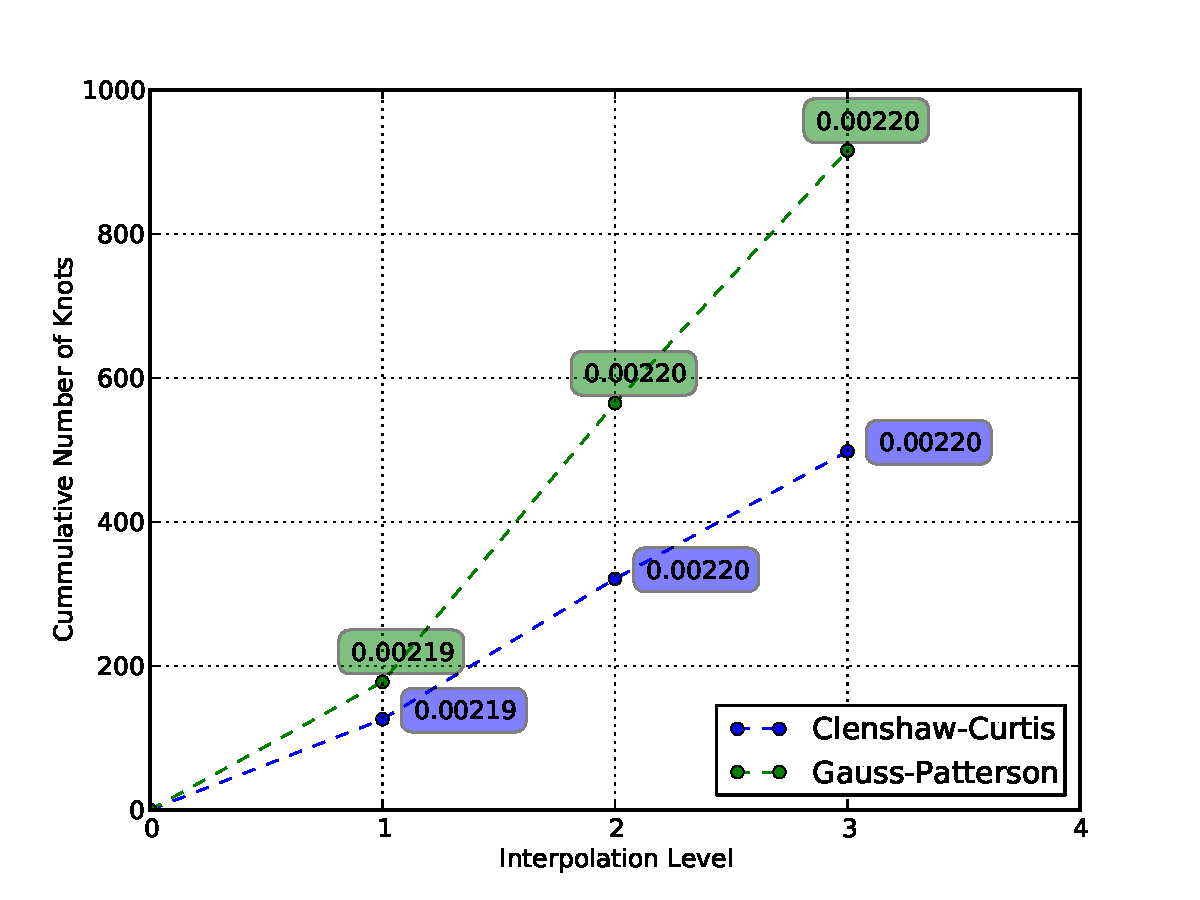
\includegraphics[scale=.75]{./Chapter3/pk_sparse_grid_numknots.pdf}
 \end{center}
\end{figure}
The Gauss-Patterson scheme required almost twice as many knots as Clenshaw-Curtis to adaptively build the reduced order model. From Figure \ref{fig:pk_sparse_grid_numknots} it's clear that the reduced order model consisting of only one dimensional components is effectively just as accurate as the full model, but requiring only 126 function evaluations to build using Clenshaw-Curtis. To see how well the reduced order models are able to reproduce the mean and variance of the true function Monte Carlo simulation is utilized. The models produced using anchored-\ac{ANOVA} decomposition with superposition dimensions of one and three are sampled along with the true function. Mean, variance, and pertinent 99\% confidence intervals for the sampling are summarized in Table \ref{table:pk_mean_variance}. A total of 1000 samples were used for each method, each using the same random numbers.      
\begin{table}[!htb] 
\caption{\label{table:pk_mean_variance} 
Mean and variance data for the maximum fuel temperature achieved during transient obtained using Monte Carlo sampling. The same random numbers were used for all 1000 samples for each method.}
\centering
\small
\begin{tabular}{||c|c|c|c|c||} 
\hline \hline
\textbf{Method} & \textbf{Mean} & \textbf{99\% CI} & \textbf{Standard Dev.} & \textbf{99\% CI} \\ \hline
1D ANOVA CC  & 1.03193 & (1.03175, 1.03211) & 0.002187 & (0.002068, 0.002320) \\ \hline
All ANOVA CC & 1.03193 & (1.03175, 1.03211) & 0.002196 & (0.002076, 0.002330) \\ \hline
1D ANOVA GP  & 1.03193 & (1.03175, 1.03211) & 0.002187 & (0.002068, 0.002320) \\ \hline
All ANOVA GP & 1.03193 & (1.03175, 1.03211) & 0.002196 & (0.002076, 0.002330) \\ \hline
True Function & 1.03193 & (1.03175, 1.03211) & 0.002196 & (0.002076, 0.002330) \\ 
\hline \hline
\end{tabular}
\end{table}
As evidenced in Table \ref{table:pk_mean_variance} the statistical results for each method are consistent. While the reduced order model with superposition dimension of three is able to replicate the Monte Carlo results to five significant figures, the expected accuracy, the order-one superposition model is slightly short. Of course, this is due to the absence of higher order components. However, the proximity of the order-one superposition model's results to the true results indicate that for this problem the higher order components do not have a significant impact. To further verify the ability of the reduced order models to accurately reproduce basic statistical moments, the probability distributions for the normalized maximum fuel temperature produced by each model are compared in Figure \ref{fig:pk_histograms}. 
\begin{figure}[!htb]
\caption{\label{fig:pk_histograms}
Histograms produced by sampling the true function, order-one superposition reduced order model, and the full adaptive reduced order model.  
}
 \begin{center}
  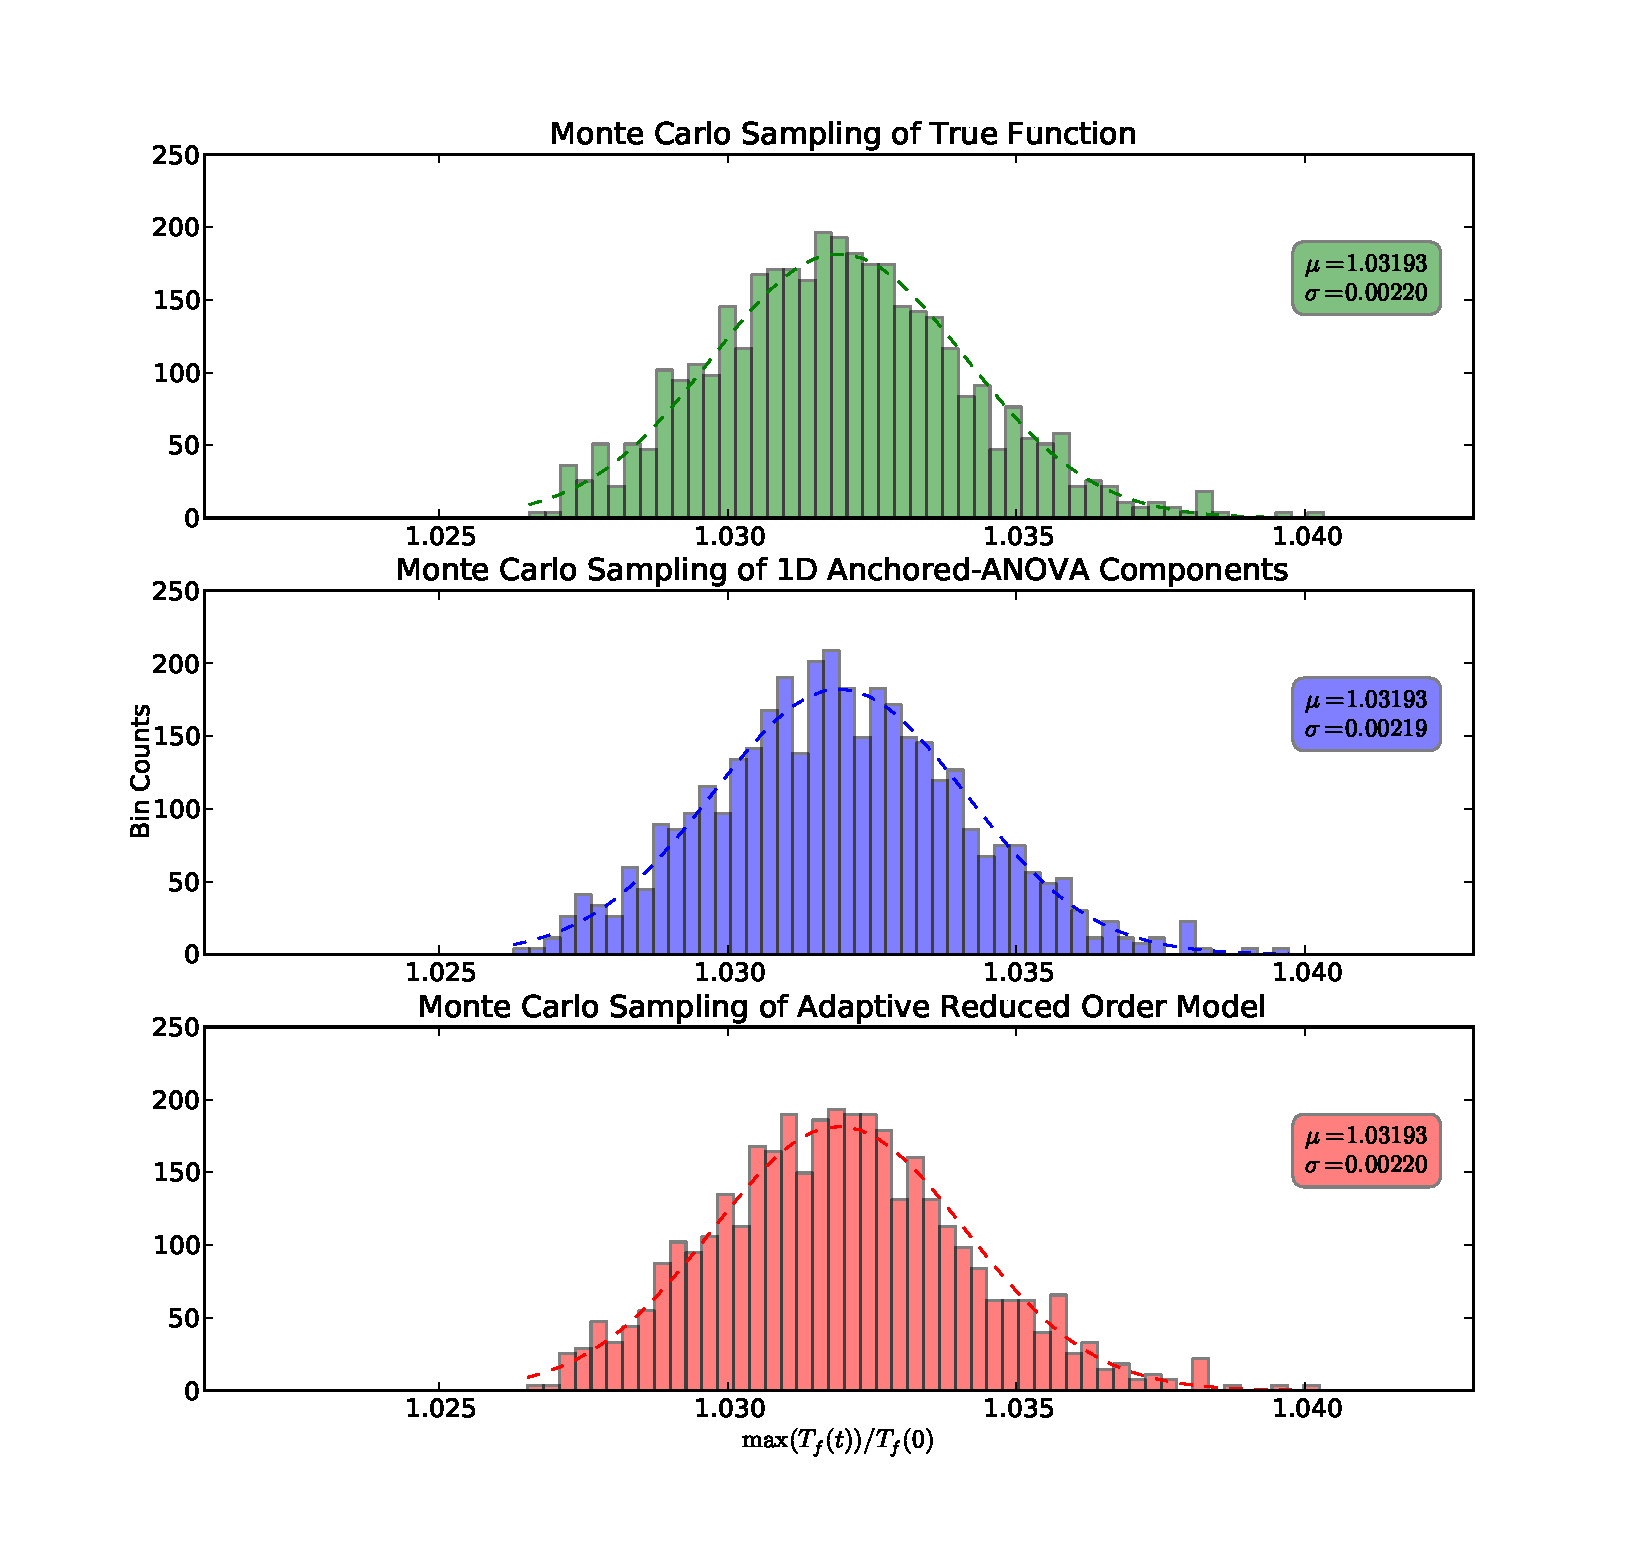
\includegraphics[scale=.58]{./Chapter3/pk_histograms.pdf}
 \end{center}
\end{figure}
All of the tested reduced order models are able to reproduce the Gaussian probability distribution for the normalized maximum fuel temperature. 

As done in section \ref{subsec:kinf_analysis}, a sensitivity analysis will be completed for the reduced order model and compared to the normalized sensitivity coefficients obtained using central differencing. From Table \ref{table:pk_sensitivities} notice that the largest sensitivity coefficients are those of the random variables deemed "important" using the adaptive reduced order model algorithm. Only the sensitivity coefficients for the Clenshaw-Curtis sparse grid are shown in Table \ref{table:pk_sensitivities} since the Gauss-Patterson sparse grid returns identical results. The normalized sensitivity coefficients calculated using the reduced order models are the same as those calculated using central differencing to the expected number of significant digits.   
\begin{table}[!htb] 
\caption{\label{table:pk_sensitivities} 
Normalized sensitivity coefficients of the maximum fuel temperature to random variables.}
\centering
\begin{tabular}{||c|c|c|c||} 
\hline \hline
\textbf{Random Variable} & \textbf{1D ANOVA CC} & \textbf{All ANOVA CC} & \textbf{Central Diff.} \\ \hline
$\lambda_1$  &  3.7894E-05 &  3.7894E-05 &  3.7895E-05 \\ \hline
$\lambda_2$  &  7.0387E-04 &  7.0387E-04 &  7.0387E-04 \\ \hline
$\lambda_3$  &  8.4244E-04 &  8.4244E-04 &  8.4215E-04 \\ \hline
$\lambda_4$  &  9.7308E-04 &  9.7309E-04 &  9.7379E-04 \\ \hline
$\lambda_5$  &  1.1572E-04 &  1.1572E-04 &  1.1607E-04 \\ \hline
$\lambda_6$  &  4.4638E-05 &  4.4639E-05 &  4.0498E-05 \\ \hline
$\beta_1$    & -3.2992E-04 & -3.2992E-04 & -3.2976E-04 \\ \hline
$\beta_2$    & -2.6582E-03 & -2.6582E-03 & -2.6616E-03 \\ \hline
$\beta_3$    & -1.1953E-03 & -1.1953E-03 & -1.2040E-03 \\ \hline
$\beta_4$    & -1.0129E-03 & -1.0129E-03 & -1.0232E-03 \\ \hline
$\beta_5$    & -1.1689E-04 & -1.1689E-04 & -1.1810E-04 \\ \hline
$\beta_6$    & -4.0718E-05 & -4.0718E-05 & -4.1134E-05 \\ \hline
$\Lambda$    & -8.9294E-08 & -8.9295E-08 & -8.9364E-08 \\ \hline
$Ah$         &  1.2553E-02 &  1.2553E-02 &  1.2584E-02 \\ \hline
$M_c$        &  1.8753E-03 &  1.8753E-03 &  1.8716E-03 \\ \hline
$M_f$        & -3.6695E-04 & -3.6695E-04 & -3.6360E-04 \\ \hline
$c_{pc}$     &  1.8753E-03 &  1.8753E-03 &  1.8903E-03 \\ \hline
$c_{pf}$     & -3.6695E-04 & -3.6695E-04 & -3.5976E-04 \\ \hline
$v$          &  1.8838E-03 &  1.8839E-03 &  1.9177E-03 \\ \hline
$\alpha_d $  & -2.6655E-02 & -2.6656E-02 & -2.6625E-02 \\ \hline
$\alpha_c$   &  8.4387E-04 &  8.4387E-04 &  8.7194E-04 \\ \hline
$\rho_{max}$ &  3.1164E-02 &  3.1164E-02 &  3.1272E-02 \\ 
\hline \hline
\end{tabular}
\end{table}

